\documentclass[letter,11pt,oneside]{article}

%%% (occur "\\(\\\\[a-z]*section\\|appendix\\|input\\|\\<include\\>\\)")

%%\documentclass[11pt,twocolumn]{article}
%%\usepackage[inline]{asymptote}   %% Inline asymptote diagrams
%%\usepackage{wglatex}             %% Use this one and kill others.
\usepackage{color}               %% colored letters {\color{red}{{text}}
\usepackage{fancyhdr}            %% headers/footers
%%\usepackage{fancyvrb}            %% headers/footers
\usepackage{datetime}            %% pick up tex date time 
\usepackage{lastpage}            %% support page of ...lastpage
\usepackage{times}               %% native times roman fonts
\usepackage{textcomp}            %% trademark
\usepackage{amssymb,amsmath}     %% greek alphabet
\usepackage{parskip}             %% blank lines between paragraphs, no indent
\usepackage{shortvrb}            %% short verb use for tables
\usepackage{lscape}              %% landscape for tables.
\usepackage{longtable}           %% permit tables to span pages wg-longtable
\usepackage{url}                 %% Make URLs uniform and links in PDFs
\usepackage{enumerate}           %% Allow letters/decorations for enumerations
\usepackage{endnotes}            %% Enhance footnotes/endnotes
\usepackage{listings}            %% Make URLs uniform and links in PDFs
\pdfadjustspacing=1                %% force LaTeX-like character spacing
\usepackage{geometry}            %% allow margins to be relaxed
%%\usepackage{wrapfig}             %% permit wrapping figures.
%%\usepackage{subfigure}              %% images side by side.
\geometry{margin=1in}            %% Allow narrower margins etc.
\usepackage[T1]{fontenc}         %% Better Verbatim Font.
\renewcommand*\ttdefault{txtt}   %% 
%%\usepackage{natbib}   %% bibitems

%% include background image (wg-document-page-background) 

\usepackage{graphicx}            %% Include pictures into a document
%% (wg-texdoc-inserttikz)


\def\documentisdraft{NOTDRAFT}

%% (wg-texdoc-isdraft)
%% (wg-texdoc-insert-fancy-headers)

%%\usepackage[bookmarks]{hyperref} %% Make huperlinks within a PDF
%%\usepackage{makeidx}             %% Make an index uncomment following line
%%\makeindex                       %%.. yeah this one, too. index{key} in text
%%



\definecolor{verbcolor}{rgb}{0.6,0,0}
\definecolor{darkgreen}{rgb}{0,0.4,0}
\newcommand\debate[1]{\textcolor{darkgreen}{DEBATE: #1} \marginpar{\textcolor{red}{DEBATE} }}
\newcommand{\ltodo}[2]{\marginpar{\textcolor{red}{ACTION: #1}\endnote{#2}}}
\renewcommand{\thefigure}{\thesection-\arabic{figure}}
\newcommand{\menu}{\ensuremath{\;\rightarrow\;}}
%%(wg-add-inline-images)  %% add inline images to the mix





%%(%%Begin User Definitions: Hint: ~/.latex.defs and  latex.defs  
%%End User Definitions:wg-texdoc-adjust-paper-width)
%% (wg-texdoc-insert-hypersetup)



%%%%%%%%%%%%%%%%%%%%%%%%%%%%%%%%%%%%%%%%%%%%%%%%%%%%%%%%%%%%%%%%%%%%%%%%%%%%%


\begin{document}


%% (wg-latex-pretty-title-page)
%% (wg-texdoc-titleblock)

\setcounter{section}{0}
\pagenumbering{arabic}

\ifx\documentisdraft\drafttest
\linenumbers    %%%%%%%%%%%%% DRAFT
\fi

\section{XEphem Parallactic Angle}




%%\appendix
%%\renewcommand \thesection{\Alph{section}}
/opt/io/wayne/clones/xephem/xephem-3.7.6-RC2/libastro/
parallactic.c
misc.c

\begingroup \fontsize{10pt}{10pt}
\selectfont
%%\begin{Verbatim} [commandchars=\\\{\}]
\begin{verbatim} 


/* solve a spherical triangle:
 *           A
 *          /  \
 *         /    \
 *      c /      \ b
 *       /        \
 *      /          \
 *    B ____________ C
 *           a
 *
 * given A, b, c find B and a in range 0..B..2PI and 0..a..PI, respectively..
 * cap and Bp may be NULL if not interested in either one.
 * N.B. we pass in cos(c) and sin(c) because in many problems one of the sides
 *   remains constant for many values of A and b.
 */

void solve_sphere (double A, double b, double cc, double sc, double *cap, double *Bp)
{
   double cb = cos(b), sb = sin(b);
   double sA, cA = cos(A);
   double x, y;
   double ca;
   double B;

   ca = cb*cc + sb*sc*cA;

   if (ca >  1.0) ca =  1.0;
   if (ca < -1.0) ca = -1.0;
   if (cap)
      *cap = ca;

   if (!Bp)
      return;

   if (sc < 1e-7)
      B = cc < 0 ? A : PI-A;
   else
   {
      sA = sin(A);
      y = sA*sb*sc;
      x = cb - ca*cc;
      B = y ? (x ? atan2(y,x) : (y>0 ? PI/2 : -PI/2)) : (x>=0 ? 0 : PI);
    }

    *Bp = B;
    unwrap_angle (Bp, 2*PI);
} /* solve_sphere */


/* compute parallactic angle given latitude, object dec and alt.
 * all angles in rads.
 * N.B. always return >= 0, caller must determine sign and degenerate cases at
 *   pole or zenith.
 */
double
parallacticLDA (double lt, double dec, double alt)
{
	double ca = sin(lt);
	double cb = sin(dec);
	double sb = cos(dec);
	double cc = sin(alt);
	double sc = cos(alt);
	double cpa;

	/* given three sides find an angle */
	if (sb==0 || sc==0)
	    return (0);
	cpa = (ca - cb*cc)/(sb*sc);
	if (cpa < -1) cpa = -1;
	if (cpa >  1) cpa =  1;
	return (acos (cpa));
}

/* compute parallactic angle given latitude, object HA and Dec.
 * all angles in rads.
 * return value is between -PI and PI, sign is like HA, ie +west
 */
double
parallacticLHD (double lt, double ha, double dec)
{
	double A, b, cc, sc, B;

	A = ha;
	b = PI/2 - lt;
	cc = sin(dec);
	sc = cos(dec);
	solve_sphere (A, b, cc, sc, NULL, &B);

	if (B > PI)
	    B -= 2*PI;
	return (B);
}

/* insure 0 <= *v < r.
 */
void
range (double *v, double r)
{
	*v -= r*floor(*v/r);
}

\end{verbatim}
\endgroup
%% \end{Verbatim}

\section{Degenerate Cases}

The poles and the zenith are difficult. The zenith is approximating
ideal airmass and very low diffraction to begin with.

When does the airmass or dispersion make a difference.

\section{Sellmeier Equation Atmospheric Dispersion}

There are quite a few issues wrapped up in this: one
is the fact the refractive index of air $n_{\rm{air}}$ varies
with composition, pressure and temperature -- all gradients
in the local atmosphere.

This is a similar form of the Sellmeier equation:



\begin{align}
n(\lambda) &= 1+\delta(\lambda) = 1+\sum_j\frac{K_j\,\lambda^2}{\lambda^2 - L_j}
\end{align}

\begin{align}
n^{2} &= 1+\sum_{n:1..3}\Bigr ( \frac{B_{n}\lambda^{2}}{\lambda^{2}-C_{n}} \Bigl )
\end{align}

Note: Makes use of Kramers-Kronig relationships (valid for complex
equations in the first quadrant.)

Where: $B_{n}$ are the oscillator strengths of transitoins and $C_{n}$ are
the coefficients of the suqare of the respective transition energies. 

Note: optical glass manufacturer's specifications often think of Air
at 25C and 101.325 kPa to have a "refractive index" DEFINED as precisely 1,


\begin{figure}[h!]
\centering
%%\phantomsection
%%\addcontentsline{toc}{section}{}
%%\caption{} %% \caption{{\tiny{citation}}} 
%%\includepdf[angle=90,width=\textwidth]{}); %% with package pdfpages
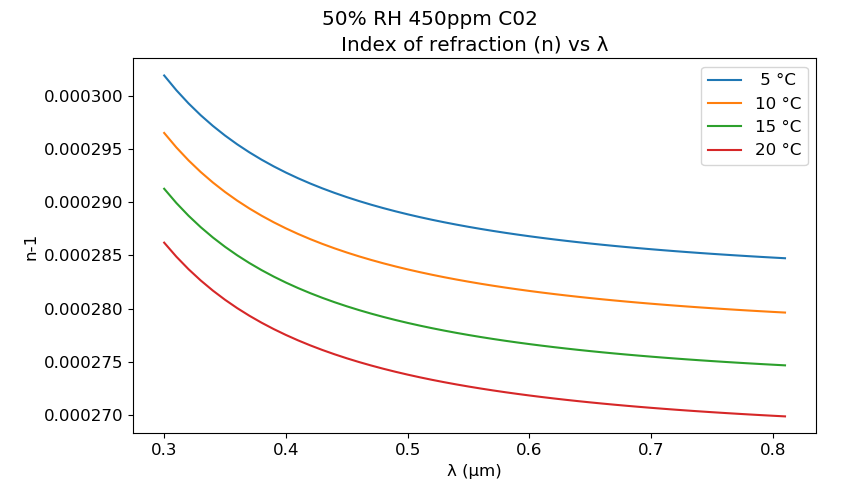
\includegraphics[width=\textwidth]{images/IndexRefraction_by_temperature.png}
\caption{Index of refraction, sealevel (101 kPa), nominal pollution. The temerature
is significant and non-linear.} %% \caption{{\tiny{citation}}} 
\label{figure:}
\end{figure}

%%%%%%%%%%%%%%%%%%%%%%%%%%%%%%%%%%%%%%%%%%%%%%%%%%%%%%%%%%%%%%%%%%%%%%%%%%%%%
%%%%%%%%%%%%%%%%%%%%%%%%%%%%%%%%%%%%%%%%%%%%%%%%%%%%%%%%%%%%%%%%%%%%%%%%%%%%%
%%%%%%%%%%%%%%%%%%%%%%%%%%%%%%%%%%%%%%%%%%%%%%%%%%%%%%%%%%%%%%%%%%%%%%%%%%%%%
%%%%%%%%%%%%%%%%%%%%%%%%%%%%%%%%%%%%%%%%%%%%%%%%%%%%%%%%%%%%%%%%%%%%%%%%%%%%%


%% use a bibitem approach to the references publications etc.
%% (wg-bibitem)

%%\clearpage
%%\addcontentsline{toc}{section}{References}
%%\renewcommand*{\refname}{My Bibliography and References}
%%\bibliographystyle{plain}	% bibliographystyle{apalike} and \usepackage{natbib}
%%\bibliography{MasterBib}	% expects file "MasterBib.bib"


%%\clearpage
%%\addcontentsline{toc}{section}{Index}
%%\printindex %% www.cs.usask.ca/resources/tutorials/latex/notes/toc-index.pdf

%%\begin{thebibliography}{80}
%%\usepackage{natbib}   %% bibitems
%%\end{thebibliography}

% /home/wayne/iraf/sasiraf/doc/p_angle.tex

%% (wg-texdoc-endnotes)
\end{document}
